\documentclass[a4paper,12pt]{article}
\usepackage[french]{babel}
\usepackage[utf8]{inputenc}
\usepackage[T1]{fontenc}
\usepackage{lmodern}
\usepackage[margin=2.54cm]{geometry}
\usepackage{amsmath,amssymb}
\usepackage{graphicx}
\usepackage{booktabs}
\usepackage{float}
\usepackage{fancyhdr}
\usepackage{cite}
\usepackage{url}
\usepackage{eso-pic}
\usepackage{caption}
\usepackage{tikz}
\usetikzlibrary{arrows}
\usepackage[colorlinks=true,linkcolor=blue,urlcolor=blue,citecolor=blue,anchorcolor=blue]{hyperref}

\setlength\parindent{0pt}
\captionsetup[table]{name=Tableau}
\captionsetup[figure]{name=Figure}

\definecolor{LightGray}{gray}{0.9}
\definecolor{LightRed}{rgb}{1.0, 0.92, 0.92}
\definecolor{LightGreen}{rgb}{0.92, 1.0, 0.92}

\graphicspath{{Image/}}

\pagestyle{fancy}
\fancyhf{}
\fancyhead[L]{8INF950: Mapping base de données d'incidents}
\fancyhead[R]{\today}
\fancyfoot[R]{\thepage}

\newcommand{\AddLogoTopRight}{
  \AddToShipoutPictureBG*{
    \ifnum\value{page}=1
      \put(\LenToUnit{0.32\paperwidth},\LenToUnit{0.75\paperheight}){%
        
\includegraphics[width=8cm]{logo-uqac.eps}%
      }
    \fi
  }
}

\begin{document}
%\AddLogoTopRight

\begin{titlepage}
    \centering
	
\includegraphics[width=8cm]{logo-uqac.eps}\\[1cm]
    \vspace*{2cm}
    {\large\bfseries Module d'informatique et de mathématique \\
    Département d'informatique et de mathématiques \par}
    {\Huge\bfseries -------------------------- \par}
    \vspace{2cm}
    {\large\bfseries 8INF950: Sujet spécial en cybersécurité \par}
    \vspace{1cm}
    {\large\bfseries Cybersécurité défensive: Mapping automatique de base de données d'incident et de détection \par}
    \vfill
    {\large Date: \today \par}
    {\large 8INF950: Sujet spécial en cybersécurité - Été 2026 \par}
\end{titlepage}

\newpage
\tableofcontents
\listoffigures
\newpage

% =============================================================================
% Auteurs : XXXXXXXXXXX
% =============================================================================
%
% --- §1 LECTURE ---
% --- PAGE DE TITRE ---
% --- §2 INTRODUCTION ---
% -> Relire / refaire toute la partie introduction
% --- §3 MÉTHODOLOGIE ---
% -> Relire / refaire toute la partie introduction
% --- §4 SOLUTION ---
% -> Relire la partie RAG 
% --- §5 RÉSULTATS ---
% -> à implémenter 
% --- §6 DISCUSSION ---
% -> à implémenter 
% --- §7 CONCLUSION ---
% -> à implémenter 

% =============================================================================
% FIN TODO RELECTURE
% =============================================================================

\section{Synthèse des lectures}

\subsection{Doc 1 — 99\% de faux positifs}

On distingue trois types de faux positifs (FP)~:
\begin{itemize}
    \item \textbf{Vraies alarmes :} ce sont les menaces réelles.
    \item \textbf{Fausses alarmes :} le système se déclenche sans raison légitime.
    \item \textbf{Alarmes bénignes :} alarmes techniquement correctes, mais
          correspondant à un comportement légitime.
\end{itemize}

La validation des alarmes repose encore sur un processus humain, grâce aux
connaissances et à l'expérience des analystes.

Les auteurs proposent le modèle \textbf{REACT} : les alarmes doivent être
\begin{itemize}
    \item \textbf{R}eliable (fiables) ;
    \item \textbf{E}xplained (explicables) ;
    \item \textbf{A}nalytical (analytiques) ;
    \item \textbf{C}ontextual (contextuelles) ;
    \item \textbf{T}ransferable (transférables à d'autres environnements).
\end{itemize}
Ce modèle est pensé pour guider la conception d'outils fondés sur
l'apprentissage automatique.

\subsection{Doc 2 — UCO (Unified Cybersecurity Ontology)}

UCO est une ontologie sémantique visant à unifier et intégrer les données
hétérogènes de cybersécurité issues de multiples standards. Son but est
d'\emph{améliorer la conscience situationnelle des analystes}.

Caractéristiques principales~:
\begin{itemize}
    \item Extension de l'ontologie IDS développée par le même groupe.
    \item Intégration des standards les plus utilisés en cybersécurité~:
          STIX, CVE, CCE, CVSS, CAPEC, CybOX et la \emph{Kill Chain}.
    \item Représentation en OWL/RDF plutôt qu'en XML, ce qui autorise le
          raisonnement automatique.
    \item 106 classes, 59 propriétés d'objet et 45 propriétés de données.
    \item Expressivité logique de niveau $\mathcal{ALCROIQ}(D)$.
\end{itemize}

\paragraph{Apport.}
Inférence logique, mappée au \emph{Linked Open Data} (DBpedia, YAGO, etc.),
permettant le croisement des données cyber avec des connaissances générales.

\paragraph{Cas d'usage.}
Un prototype identifie les vulnérabilités liées à un type de logiciel à partir
des données NVD. Au moyen de requêtes SPARQL, il recense les produits d'un
éditeur et leurs vulnérabilités, afin de suggérer une alternative exempte de
vulnérabilités ou de comparer l'impact sécuritaire d'un changement de
fournisseur.

\newpage
%==============================================================================
\section{Introduction}
%==============================================================================

\subsection{Problématique et objectifs}

Dans un centre d'opérations de sécurité (SOC), les analystes doivent constamment relier
des incidents décrits dans un vocabulaire normalisé aux techniques adverses documentées
dans des référentiels offensifs. Ce travail d'alignement sémantique permet d'enrichir la détection,
contextualiser les alertes et améliorer la conscience
situationnelle, mais il reste en grande partie manuel, coûteux et peu
reproductible.

L'objectif de ce projet est de reproduire automatiquement, à l'aide de
l'intelligence artificielle, le mapping entre le vocabulaire VERIS et le
framework MITRE ATT\&CK, puis de mesurer la qualité des mappings produits par
rapport à la référence officielle publiée par le CTID (\emph{Mappings Explorer}).

Nous avons choisi de mettre trois approches en concurrence~: \newline
\textbf{- Un modèle RAG} (Retrieval-Augmented Generation)\newline
\textbf{- Un modèle d'ia modifié pour être fine-tuné} (fine-tuning supervisé) \newline
\textbf{- Un modèle d'ia généraliste avec prompt engineering} (ingénierie de prompts).\newline
\newline
Le but de notre contribution est de venir créer:
\begin{itemize}
    \item Un pipeline reproductible permettant de générer les mappings entre VERIS et MITRE ATT\&CK (préparation des données, génération, comparaison) ;
    \item Un format de sortie standardisé pour les mappings générés par nos solutions ;
    \item Des scripts de comparaison automatisée entre le mapping existant et les mappings générés par nos solutions ;
\end{itemize}

Le rapport s'organise comme suit : \newline 
- L'introduction présente le contexte technique (§\ref{sec:contexte-veris} à §\ref{sec:contexte-formats})~; \newline
- La méthodologie décrit la pratique actuelle, l'état de l'art et notre cadre expérimental~; \newline
- La section \emph{Solution} détaille les trois approches retenues~; \newline
- Les résultats, la discussion et la conclusion clôturent l'analyse. \newline

\subsection{Contexte --- VERIS}
\label{sec:contexte-veris}

VERIS (\emph{Vocabulary for Event Recording and Incident Sharing}) est un vocabulaire structuré conçu pour décrire de manière homogène les incidents de cybersécurité. Son objectif principal est de fournir un cadre commun pour documenter ce qui s'est produit lors d'un incident, indépendamment de l'organisation ou de l'outil utilisé. Autrement dit, VERIS sert à normaliser la description des événements de sécurité afin de faciliter leur analyse, leur comparaison et leur partage entre analystes, équipes de réponse à incident et organismes de recherche.

Sur le plan de son organisation, VERIS repose sur une structure hiérarchique. Le vocabulaire est découpé en grands axes, comme \texttt{action}, \texttt{attribute}, \texttt{actor} ou encore \texttt{value\_chain}, qui correspondent à différentes dimensions d'un incident. Chaque axe contient ensuite des catégories plus précises, par exemple \texttt{hacking}, \texttt{malware} ou \texttt{social} dans l'axe \texttt{action}, puis des sous-catégories et des valeurs plus fines telles que \texttt{variety} ou \texttt{vector}. Cette organisation permet de représenter un incident avec plusieurs niveaux de granularité, depuis une vue générale jusqu'à une description beaucoup plus détaillée du comportement observé.

VERIS a été développé à l'origine dans le cadre des travaux de Verizon autour du \emph{Data Breach Investigations Report} (DBIR), avec l'idée de disposer d'un schéma cohérent pour collecter et comparer les données d'incidents à grande échelle. Avec le temps, il est devenu un standard largement reconnu dans le domaine de la réponse à incident et de l'analyse cyber, notamment parce qu'il permet d'agréger des observations provenant de sources variées tout en conservant une structure commune. Dans le cadre de ce projet, VERIS joue donc le rôle de référentiel décrivant le ``quoi'' de l'incident, que l'on cherche ensuite à relier au ``comment'' représenté par les techniques de MITRE ATT\&CK.

\subsection{Contexte --- MITRE ATT\&CK}

\textbf{MITRE ATT\&CK} (\emph{Adversarial Tactics, Techniques, and Common Knowledge}) est une base de connaissances dédiée à la description des comportements adverses observés lors d'intrusions réelles. Contrairement à un simple catalogue de vulnérabilités ou d'outils, ATT\&CK cherche à modéliser la manière dont un attaquant agit au cours d'une opération, c'est-à-dire les étapes, les objectifs intermédiaires et les techniques mobilisées. Dans cette perspective, ATT\&CK décrit le ``comment'' d'une attaque, là où d'autres référentiels, comme VERIS, décrivent davantage le ``quoi'' de l'incident.

Le framework est organisé de manière hiérarchique autour de \textbf{tactiques} et de \textbf{techniques}. Les tactiques représentent les grands objectifs poursuivis par l'attaquant, par exemple l'accès initial, l'exécution, la persistance, l'élévation de privilèges ou l'impact. À l'intérieur de chaque tactique, ATT\&CK recense des techniques identifiées par un code de type \texttt{T1059}, accompagnées d'un nom, d'une description et d'un ensemble de tactiques associées. Certaines techniques sont elles-mêmes décomposées en \textbf{sous-techniques}, notées par exemple \texttt{T1059.001}, ce qui permet de représenter plus finement des variantes de comportement ou des modes opératoires particuliers.

MITRE ATT\&CK est maintenu par la MITRE Corporation à partir de retours d'expérience opérationnels, de rapports d'incidents et d'observations issues du renseignement sur les menaces. Il s'est progressivement imposé comme une référence majeure en cybersécurité défensive, notamment pour la détection, la chasse aux menaces, l'évaluation de couverture et la structuration des connaissances sur les attaques. Dans le cadre de ce projet, ATT\&CK constitue le référentiel cible vers lequel les capacités VERIS sont mappées, afin de relier la description d'un incident aux techniques adverses susceptibles d'en expliquer le déroulement.

\subsection{Contexte --- Le mapping}

Le mapping étudié dans ce projet consiste à relier des capacités issues du vocabulaire VERIS, qui décrivent la nature et les caractéristiques d'un incident, à des techniques du framework MITRE ATT\&CK, qui décrivent les comportements et modes opératoires adverses susceptibles d'expliquer cet incident. Autrement dit, il s'agit de faire le lien entre le ``quoi'' observé dans VERIS et le ``comment'' modélisé dans ATT\&CK. Concrètement, une capacité VERIS, par exemple \texttt{action.hacking.variety.SQLi}, peut être associée à une ou plusieurs techniques ATT\&CK jugées pertinentes par les experts.

Ces correspondances sont produites et publiées par le CTID / MITRE Engenuity. Elles constituent dans notre travail une double référence : d'une part, elles définissent la cible que nos solutions d'intelligence artificielle cherchent à reproduire automatiquement ; d'autre part, elles servent de base d'évaluation pour mesurer la qualité des mappings générés. Le problème traité dans ce projet n'est donc pas seulement de produire des associations plausibles entre VERIS et ATT\&CK, mais bien de se rapprocher le plus possible d'un mapping expert déjà établi.

\subsection{Contexte --- Les 7 capability groups}

Sept groupes VERIS dits «~comportementaux~» sont mappés vers ATT\&CK. Le
Tableau~\ref{tab:capability-groups} présente les volumes pour la paire de référence
VERIS~1.4.1 / ATT\&CK~19.1.

\begin{table}[H]
  \centering
  \begin{tabular}{l r r}
    \toprule
    \textbf{Capability group} & \textbf{Paires VERIS$\leftrightarrow$ATT\&CK} & \textbf{Capacités VERIS} \\
    \midrule
    \texttt{action.hacking}            & 538 & 68 \\
    \texttt{action.malware}              & 405 & 54 \\
    \texttt{action.social}             &  78 & 23 \\
    \texttt{attribute.integrity}       &  91 & 13 \\
    \texttt{attribute.confidentiality} &  73 &  1 \\
    \texttt{attribute.availability}    &  44 &  6 \\
    \texttt{value\_chain.development}  &  25 & 12 \\
    \bottomrule
  \end{tabular}
  \caption{Les sept capability groups VERIS mappés (référence 1.4.1 / 19.1).}
  \label{tab:capability-groups}
\end{table}

\noindent
\textit{Cas particulier~:} pour \texttt{attribute.confidentiality}, les experts mappent
le champ \texttt{data\_disclosure} lui-même (une seule capacité), et non des valeurs
sous \texttt{variety}.

\subsection{Contexte --- Versions et formats de données}
\label{sec:contexte-formats}

Quatre paires de versions sont supportées de bout en bout~: 
ATT\&CK~9.0 / VERIS~1.3.5,
12.1 / 1.3.7,
16.1 / 1.4.0 
et 19.1 / 1.4.1. \newline
La \textbf{version cible d'évaluation}
de ce rapport est VERIS~1.4.1 / ATT\&CK~19.1 (clé
\texttt{veris-1.4.1\_attack-19.1-enterprise}).

Les entrées préparées pour chaque solution sont~:
\begin{itemize}
    \item \texttt{veris\_<v>.json}~: capacités VERIS dans les sept groupes (les «~questions~») ;
    \item \texttt{attack\_<a>.json}~: techniques ATT\&CK non dépréciées (les «~candidats~»).
\end{itemize}
Les sorties des solutions suivent le format \texttt{veris\_to\_mitre}~; la référence
experte utilise le format CTID (\texttt{mapping\_objects}).

%==============================================================================
\section{Méthodologie}
%==============================================================================


%TODO peut etre à mettre dans l'introduction ????????????????????
\subsection{La méthode actuelle de mapping}

Aujourd'hui, le mapping VERIS $\rightarrow$ ATT\&CK est réalisé par des experts du
CTID / MITRE Engenuity~\cite{ctid_mappings}. Le processus est essentiellement
\textbf{manuel}~: pour chaque capacité VERIS, l'expert analyse sa sémantique, consulte
le catalogue ATT\&CK et sélectionne les techniques correspondantes (y compris les
sous-techniques lorsque nécessaire). Les résultats sont publiés via l'outil
\emph{Mappings Explorer} au format CTID.

Cette approche présente des \textbf{avantages} indiscutables~: haute qualité,
validation par des spécialistes et référence largement adoptée. Ses
\textbf{limites} sont toutefois significatives~: coût en temps humain, faible
scalabilité et nécessité de recommencer le travail à chaque nouvelle version de VERIS
ou d'ATT\&CK. Notre projet vise précisément à automatiser cette tâche tout en
mesurant l'écart par rapport à cette référence experte.

%TODO utile ? 
\subsection{État de l'art --- Alarmes SIEM et modèle REACT}

On distingue trois types de faux positifs (FP) dans les systèmes SIEM~\cite{react_model}~:
\begin{itemize}
    \item \textbf{Vraies alarmes}~: menaces réelles.
    \item \textbf{Fausses alarmes}~: déclenchement sans raison légitime.
    \item \textbf{Alarmes bénignes}~: techniquement correctes, mais correspondant à un comportement légitime.
\end{itemize}

La validation des alarmes repose encore largement sur l'expertise humaine. Les auteurs
proposent le modèle \textbf{REACT}~: les alarmes doivent être \textbf{R}eliable
(fiables), \textbf{E}xplained (explicables), \textbf{A}nalytical (analytiques),
\textbf{C}ontextual (contextuelles) et \textbf{T}ransferable (transférables). Ce
cadre guide la conception d'outils fondés sur l'apprentissage automatique. Dans notre
projet, l'automatisation du mapping VERIS$\leftrightarrow$ATT\&CK vise à réduire la
charge cognitive des analystes en normalisant plus rapidement le lien entre incidents
et techniques adverses.

%TODO utile ? 
\subsection{État de l'art --- Ontologies et unification (UCO)}

\textbf{UCO} (\emph{Unified Cybersecurity Ontology})~\cite{uco2015} est une ontologie
sémantique visant à unifier des données hétérogènes de cybersécurité (STIX, CVE,
CAPEC, CybOX, \emph{Kill Chain}, etc.) en OWL/RDF, ce qui autorise le raisonnement
automatique. L'alignement VERIS $\leftrightarrow$ ATT\&CK s'inscrit dans cette
problématique plus large d'\textbf{unification de taxonomies cyber}~: deux vocabulaires
distincts doivent être reliés de manière cohérente pour améliorer la conscience
situationnelle des analystes.

\subsection{État de l'art --- Approches IA pour l'alignement sémantique}

Trois familles d'approches sont comparées dans ce projet~:
\begin{itemize}
    \item \textbf{Prompt engineering}~: un LLM généraliste produit le mapping à partir
          d'instructions (zero-shot ou few-shot).
    \item \textbf{Fine-tuning}~: un modèle est entraîné sur des paires expert
          annotées. Spécialisation forte et nous supposons une faible hallucination, mais avec un coût
          d'entraînement plus élevé.
    \item \textbf{RAG}~\cite{lewis2020rag}~: un contexte pertinent (techniques ATT\&CK,
          exemples experts) est récupéré avant la décision. Compromis entre
          interprétabilité, coût et performance.
\end{itemize}

\subsection{Notre pipeline}

Notre pipeline expérimental s'organise en quatre étapes principales, illustrées à la
Figure~\ref{fig:pipeline}. L'objectif est de partir de sources officielles, de produire
des mappings automatisés VERIS $\rightarrow$ ATT\&CK à l'aide de trois approches IA, puis
de les comparer au mapping expert CTID.

\begin{figure}[H]
  \centering
  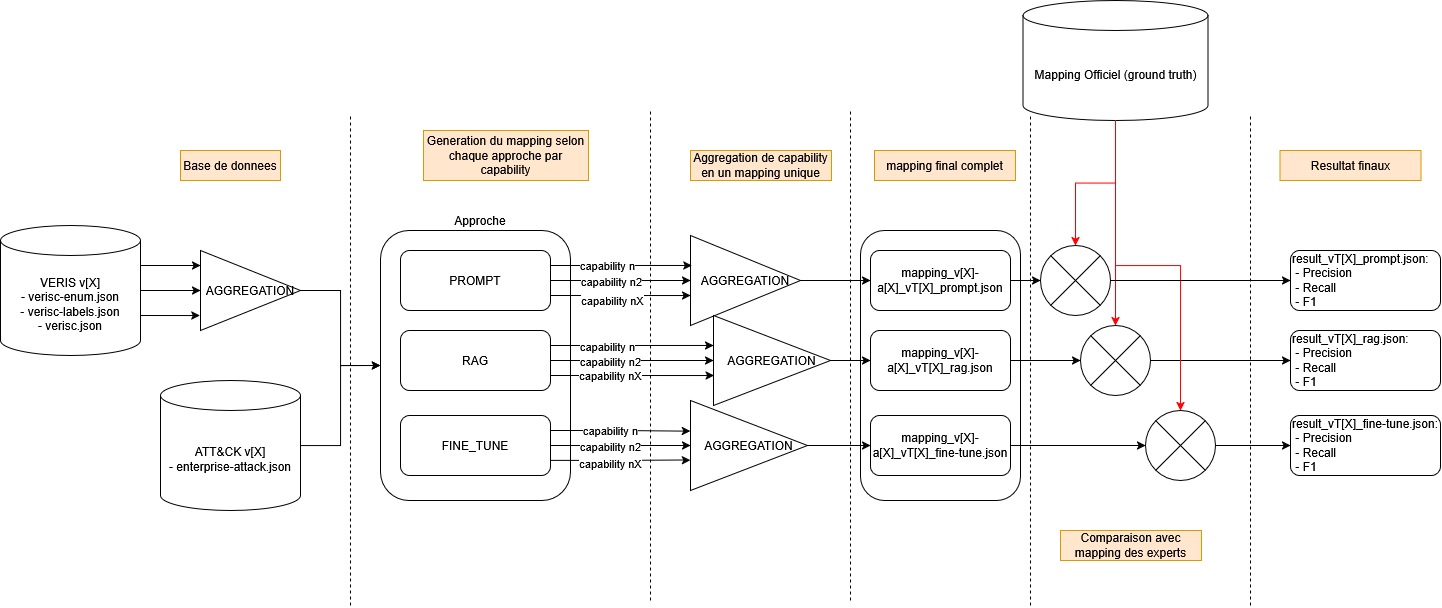
\includegraphics[width=0.92\linewidth]{schema_du_pipeline.png}
  \caption{Pipeline global du projet~: données brutes, trois solutions IA et comparaison aux experts.}
  \label{fig:pipeline}
\end{figure}

\begin{enumerate}
    \item \textbf{Téléchargement des données brutes.}
          Les sources officielles sont rassemblées dans le dossier \texttt{data/raw/}.
          On y trouve les fichiers VERIS (\texttt{verisc-enum.json}, \texttt{verisc-labels.json},
          \texttt{verisc.json}), le catalogue ATT\&CK au format STIX
          (\texttt{enterprise-attack.json}) ainsi que les mappings experts publiés par le CTID
          (CSV, YAML, JSON ou STIX selon la version). Quatre paires de versions sont
          disponibles, de VERIS~1.3.5 / ATT\&CK~9.0 à VERIS~1.4.1 / ATT\&CK~19.1.

    \item \textbf{Préparation des entrées.}
          Le script \texttt{tools/build\_work\_inputs.py} transforme ces données brutes en
          fichiers exploitables par les solutions IA, stockés dans \texttt{data\_for\_work/}.
          Pour chaque paire de versions, il produit~:
          \begin{itemize}
              \item \texttt{veris\_<v>.json}~: les capacités VERIS des sept capability groups
                    (les «~questions~» à mapper) ;
              \item \texttt{attack\_<a>.json}~: les techniques ATT\&CK non dépréciées
                    (les «~candidats~») ;
              \item \texttt{mapping\_des\_experts.json}~: une copie locale du mapping de
                    référence, utilisée pour la comparaison.
          \end{itemize}

    \item \textbf{Génération des mappings.}
          Chacune des trois solutions (\texttt{Solution\_RAG}, \texttt{Solution\_PROMPT},
          \texttt{Solution\_FINE\_TUNE}) ingère les fichiers préparés et produit
          \textbf{sept fichiers JSON} au format \texttt{veris\_to\_mitre}, soit un fichier par
          capability group (\texttt{action.hacking}, \texttt{action.malware},
          \texttt{action.social}, \texttt{attribute.integrity},
          \texttt{attribute.confidentiality}, \texttt{attribute.availability},
          \texttt{value\_chain.development}). Les résultats sont écrits dans
          \texttt{Resultat/Resultat\_<APPROCHE>/}.

    \item \textbf{Comparaison aux experts.}
          Le script \texttt{Resultat/compare\_veris\_mappings\_v2.py} confronte automatiquement
          les sorties des solutions au mapping expert CTID
          (\texttt{Resultat/Mapping\_des\_experts/}). Il valide la présence des sept fichiers,
          calcule les métriques de recouvrement (précision, rappel, F1, Jaccard) sur les paires
          \texttt{(veris\_id, attack\_id)} et classe les solutions entre elles.
\end{enumerate}

\noindent
\textbf{Principe anti-fuite.}
Pour la version cible d'évaluation (VERIS~1.4.1 / ATT\&CK~19.1), le mapping expert
correspondant n'est \textbf{jamais} utilisé comme exemple d'entraînement ou d'indexation
dans les solutions IA. Seules les versions antérieures (9.0, 12.1, 16.1) peuvent servir
d'exemples analogiques, notamment dans la variante RAG \texttt{with\_examples}.




\subsubsection{Architecture du projet}

Le dépôt SIEM est organisé de manière modulaire afin de séparer clairement les
données, leur préparation, l'implémentation des solutions IA et l'évaluation des
résultats. Cette organisation facilite la reproductibilité du pipeline et permet
de traiter plusieurs paires de versions VERIS / ATT\&CK dans un même cadre
expérimental.

\begin{itemize}
    \item \texttt{data/}~: contient les \textbf{sources brutes} issues des dépôts
          officiels. Le sous-dossier \texttt{raw/attack/} regroupe les catalogues
          ATT\&CK au format STIX, \texttt{raw/veris/} les schémas et énumérations VERIS,
          et \texttt{raw/mapping/} les mappings experts publiés par le CTID. Le
          dossier \texttt{databases/} regroupe également des bases SQLite auxiliaires
          utilisées pour certains vocabulaires et correspondances.

    \item \texttt{data\_for\_work/}~: regroupe les \textbf{entrées préparées} pour
          chaque paire de versions, dans des sous-dossiers nommés selon la convention
          \texttt{attack-<a>\_veris-<v>}. Chaque dossier contient les fichiers
          \texttt{veris\_<v>.json} (capacités VERIS à mapper),
          \texttt{attack\_<a>.json} (techniques ATT\&CK candidates) et
          \texttt{mapping\_des\_experts.json} (copie locale de la référence experte).

    \item \texttt{tools/}~: regroupe les \textbf{scripts de préparation et de
          validation} du pipeline. Le script \texttt{build\_work\_inputs.py} transforme
          les données brutes en fichiers exploitables dans
          \texttt{data\_for\_work/}, tandis que \texttt{build\_example\_results.py}
          génère des sorties de référence au format \texttt{veris\_to\_mitre}, utiles
          pour valider le format attendu.

    \item \texttt{Solution/}~: contient le \textbf{code des trois approches IA}
          mises en concurrence~: \texttt{Solution\_RAG}, \texttt{Solution\_PROMPT} et
          \texttt{Solution\_FINE\_TUNE}. Chaque solution lit les mêmes entrées
          préparées et produit sept fichiers JSON, un par capability group VERIS.

    \item \texttt{Resultat/}~: centralise les \textbf{sorties expérimentales} et les
          outils de comparaison. On y trouve les mappings experts officiels dans
          \texttt{Mapping\_des\_experts/}, les résultats produits par chaque approche
          dans \texttt{Resultat\_RAG/}, \texttt{Resultat\_PROMPT/} et
          \texttt{Resultat\_FINE\_TUNE/}, ainsi que les scripts
          \texttt{compare\_veris\_mappings.py} et
          \texttt{compare\_veris\_mappings\_v2.py} utilisés pour mesurer la qualité
          des mappings générés.
\end{itemize}

\noindent
Cette architecture matérialise le flux décrit précédemment~: les données brutes
sont d'abord normalisées, puis transformées en entrées de travail, ensuite traitées
par les solutions IA, et enfin comparées au mapping expert CTID.

%==============================================================================
\section{Solution}
%==============================================================================

Les trois solutions partagent les mêmes entrées (\texttt{veris\_<v>.json},
\texttt{attack\_<a>.json}) et la même sortie attendue (sept fichiers
\texttt{veris\_to\_mitre}), mais diffèrent par leur stratégie de décision IA.

\subsection{Solution RAG}

\subsubsection{Principe}

La solution \textbf{RAG} ancre chaque décision dans du contexte récupéré via deux
corpus vectoriels ChromaDB~:
\begin{enumerate}
    \item \texttt{attack\_techniques} --- catalogue ATT\&CK cible (les candidats) ;
    \item \texttt{expert\_examples} --- mappings experts des versions antérieures
          (exemples analogiques).
\end{enumerate}
Pour chaque capacité VERIS, le système récupère les techniques les plus similaires
(top-$k$) et, le cas échéant, des exemples de mappings experts (top-$m$), puis
produit une décision structurée en JSON.

\subsubsection{Flux par capacité VERIS}

Le traitement suit la chaîne suivante~: (1)~récupération des candidats ATT\&CK~;
(2)~récupération des exemples experts (variante \texttt{with\_examples})~;
(3)~décision via le backend configuré (\texttt{retrieval}, \texttt{local\_llm} ou
\texttt{llm} Azure)~; (4)~validation anti-hallucination (rejet des identifiants hors
catalogue)~; (5)~enrichissement des libellés et tactiques depuis le catalogue local~;
(6)~agrégation en entrées \texttt{veris\_to\_mitre} regroupées par capability group.

\subsubsection{Deux variantes expérimentées}

\begin{table}[H]
  \centering
  \begin{tabular}{l l l}
    \toprule
    \textbf{Mode} & \textbf{Corpus de récupération} & \textbf{Dossier de sortie} \\
    \midrule
    \texttt{attack\_only}   & ATT\&CK seul               & \texttt{...\_RAG\_attack\_only/} \\
    \texttt{with\_examples} & ATT\&CK + exemples experts & \texttt{...\_RAG\_with\_examples/} \\
    \bottomrule
  \end{tabular}
  \caption{Variantes expérimentées de la solution RAG.}
  \label{tab:rag-variantes}
\end{table}

\subsubsection{Modules logiciels}

\begin{table}[H]
  \centering
  \begin{tabular}{l l}
    \toprule
    \textbf{Fichier} & \textbf{Rôle} \\
    \midrule
    \texttt{config.py}           & Versions, chemins, hyperparamètres \\
    \texttt{ingest.py}           & Indexation ChromaDB \\
    \texttt{retrieve.py}         & Récupération top-$k$ / top-$m$ \\
    \texttt{prompt.py}           & Prompts et schéma JSON \\
    \texttt{generator.py}        & Backends de génération \\
    \texttt{generate\_mapping.py} & Pipeline complet $\rightarrow$ 7 fichiers \\
    \bottomrule
  \end{tabular}
  \caption{Modules principaux de la solution RAG (\texttt{veris\_mapping/}).}
  \label{tab:rag-modules}
\end{table}

\subsubsection{Technologies et configuration}

En mode local (défaut), les embeddings sont produits par \texttt{sentence-transformers}
et la génération peut s'appuyer sur la seule similarité cosinus (\texttt{retrieval}),
sans LLM. En mode Azure (optionnel), les embeddings et la génération passent par
Azure OpenAI. Les paramètres clés sont \texttt{RAG\_TOP\_K\_TECHNIQUES} (20 par défaut)
et \texttt{RAG\_TOP\_M\_EXAMPLES} (5 par défaut).

\subsubsection{Format de sortie}

Chaque fichier de résultat contient une liste \texttt{veris\_to\_mitre} avec, pour
chaque capacité, les techniques proposées, un score de confiance et une justification.
Les identifiants ATT\&CK invalides sont rejetés~; noms et tactiques proviennent du
catalogue local.

\subsection{Solution Fine-tune}

\subsection{Solution PROMPT}

\subsection{Synthèse des trois solutions}


%==============================================================================
\section{Résultats}
%==============================================================================

\subsection{Configuration expérimentale}

\subsection{Résultats --- Solution RAG}

Le Tableau~\ref{tab:rag-resultats} résume les performances globales des deux variantes
RAG. L'injection d'exemples experts des versions antérieures \textbf{double le F1}
(27,4~\% contre 9,8~\%), principalement grâce à un gain de rappel.

\begin{table}[H]
  \centering
  \begin{tabular}{l r r r}
    \toprule
    \textbf{Variante} & \textbf{Précision} & \textbf{Rappel} & \textbf{F1} \\
    \midrule
    \texttt{RAG\_with\_examples} & 18,9~\% & 49,7~\% & \textbf{27,4~\%} \\
    \texttt{RAG\_attack\_only}     &  7,2~\% & 15,4~\% &  9,8~\% \\
    \bottomrule
  \end{tabular}
  \caption{Résultats globaux RAG vs mapping expert (mode \texttt{retrieval} local).}
  \label{tab:rag-resultats}
\end{table}

Le mode \texttt{retrieval} privilégie le rappel au détriment de la précision~: de
nombreuses paires expertes sont retrouvées, mais beaucoup de propositions sont
incorrectes. Certaines familles de sous-techniques (par exemple \texttt{T1546.*})
restent partiellement couvertes lorsque le top-$k$ est insuffisant.

\subsection{Résultats --- Solution Fine-tune}


\subsection{Résultats --- Solution PROMPT}


%==============================================================================
\section{Discussion}
%==============================================================================



%==============================================================================
\section{Conclusion}
%==============================================================================


\bibliographystyle{plain}
\bibliography{biblio}

\end{document}
